%!TEX encoding = UTF-8 Unicode
\documentclass[french, a4paper, 12pt, landscape, twocolumn]{article}



%% Langue et compilation

\usepackage[utf8]{inputenc}
\usepackage[T1]{fontenc}
\usepackage[french]{babel}

%% LISTE DES PACKAGES

\usepackage{mathtools}     % package de base pour les maths
\usepackage{amsmath}       % mathematical type-setting
\usepackage{amssymb}       % symbols speciaux pour les maths
\usepackage{textcomp}      % symboles speciaux pour el text
\usepackage{gensymb}       % commandes generiques \degree etc...
\usepackage{tikz}          % package graphique
\usepackage{wrapfig}       % pour entourer a cote d'une figure
\usepackage{color}         % package des couleurs
\usepackage{xcolor}        % autre package pour les couleurs
\usepackage{pgfplots}      % pacakge pour creer des graph
\usepackage{epsfig}        % permet d'inclure des graph en .eps
\usepackage{graphicx}      % arguments dans includegraphics
\usepackage{pdfpages}      % permet d'insérer des pages pdf dans le document
\usepackage{subfig}        % permet de creer des sous-figure
\usepackage{pst-all}       % utile pour certaines figures en pstricks
\usepackage{lipsum}        % package qui permet de faire des essais
\usepackage{array}         % permet de faire des tableaux
\usepackage{multicol}      % plusieurs colonnes sur une page
\usepackage{enumitem}      % pro­vides user con­trol: enumerate, itemize and description
\usepackage{hyperref}      % permet de creer des hyperliens dans le document
\usepackage{lscape}        % permet de mettre une page en mode paysage
\usepackage{lmodern}       % permet d'avoir certains "fonts" de bonen qualite
\usepackage{fancyhdr}      % Permet de mettre des informations en hau et en bas de page      
\usepackage[framemethod=tikz]{mdframed} % breakable frames and coloured boxes
\usepackage[top=1.5cm, bottom=1.5cm, left=2.5cm, right=2.5cm]{geometry} % donne les marges
\usepackage[font=normalsize, labelfont=bf,labelsep=endash, figurename=Fig.]{caption} % permet de changer les legendes des figures
\usepackage{lewis}
\usepackage{bohr}
\usepackage{chemfig}
\usepackage{chemist}

%% LIBRAIRIES

\usetikzlibrary{plotmarks} % librairie pour les graphes
\usetikzlibrary{patterns}  % necessaire pour certaines choses predefinies sur tikz
\usetikzlibrary{shadows}   % ombres des encadres
\usetikzlibrary{backgrounds} % arriere plan des encadres


%% MISE EN PAGE

\pagestyle{fancy}     % Défini le style de la page

\renewcommand{\headrulewidth}{1pt}      % largeur du trait en haut de la page
\fancyhead[L]{Seconde générale}         % info coin haut gauche
\fancyhead[R]{Lycée Jean Guéhenno}  % info coin haut droit

% bas de la page
\renewcommand{\footrulewidth}{1pt}      % largeur du trait en bas de la page
\fancyfoot[L]{G. \bsc{LE DOUDIC}}  % info coin bas gauche
\fancyfoot[R]{TP 4 : Famille chimique}                         % info coin bas droit


\setlength{\columnseprule}{1pt} 
\setlength{\columnsep}{30pt}



%% NOUVELLES COMMANDES 

\DeclareMathOperator{\e}{e} % permet d'ecrire l'exponentielle usuellement


\newcommand{\gap}{\vspace{0.15cm}}   % defini une commande pour sauter des lignes
\renewcommand{\vec}{\overrightarrow} % permet d'avoir une fleche qui recouvre tout le vecteur
\newcommand{\bi}{\begin{itemize}}    % begin itemize
\newcommand{\ei}{\end{itemize}}      % end itemize
\newcommand{\bc}{\begin{center}}     % begin center
\newcommand{\ec}{\end{center}}       % end center
\newcommand\opacity{1}               % opacity 
\pgfsetfillopacity{\opacity}

\newcommand*\Laplace{\mathop{}\!\mathbin\bigtriangleup} % symbole de Laplace

\frenchbsetup{StandardItemLabels=true} % je ne sais plus

\newcommand{\smallO}[1]{\ensuremath{\mathop{}\mathopen{}o\mathopen{}\left(#1\right)}} % petit o

\newcommand{\cit}{\color{blue}\cite} % permet d'avoir les citations de couleur bleues
\newcommand{\bib}{\color{black}\bibitem} % paragraphe biblio en noir et blanc
\newcommand{\bthebiblio}{\color{black} \begin{thebibliography}} % idem necessaire sinon bug a cause de la couleur
\newcommand{\ethebiblio}{\color{black} \end{thebibliography}}   % idem
%%% TIKZ


%% COULEURS 


\definecolor{definitionf}{RGB}{220,252,220}
\definecolor{definitionl}{RGB}{39,123,69}
\definecolor{definitiono}{RGB}{72,148,101}

\definecolor{propositionf}{RGB}{255,216,218}
\definecolor{propositionl}{RGB}{38,38,38}
\definecolor{propositiono}{RGB}{109,109,109}

\definecolor{theof}{RGB}{255,216,218}
\definecolor{theol}{RGB}{160,0,4}
\definecolor{theoo}{RGB}{221,65,100}

\definecolor{avertl}{RGB}{163,92,0}
\definecolor{averto}{RGB}{255,144,0}

\definecolor{histf}{RGB}{241,238,193}

\definecolor{metf}{RGB}{220,230,240}
\definecolor{metl}{RGB}{56,110,165}
\definecolor{meto}{RGB}{109,109,109}


\definecolor{remf}{RGB}{230,240,250}
\definecolor{remo}{RGB}{150,150,150}

\definecolor{exef}{RGB}{240,240,240}

\definecolor{protf}{RGB}{247,228,255}
\definecolor{protl}{RGB}{105,0,203}
\definecolor{proto}{RGB}{174,88,255}

\definecolor{grid}{RGB}{180,180,180}

\definecolor{titref}{RGB}{230,230,230}

\definecolor{vert}{RGB}{23,200,23}

\definecolor{violet}{RGB}{180,0,200}

\definecolor{copper}{RGB}{217, 144, 88}

%% Couleur des ref

\hypersetup{
	colorlinks=true,
	linkcolor=black,
	citecolor=blue,
	urlcolor=black
		   }

%% CADRES


% %%%%%%%%%% DEFINITION
% \newmdenv[tikzsetting={fill=definitionf}, linewidth=2pt, linecolor=definitionl, outerlinewidth=0pt, innertopmargin=5pt, innerbottommargin=5pt, innerleftmargin=5pt, innerrightmargin=5pt, leftmargin=0pt]{definition}

% \newmdenv[ tikzsetting={drop shadow={ shadow xshift=1ex, shadow yshift=-0.5em, fill=definitiono, opacity=1, every shadow } }, outerlinewidth=2pt, outerlinecolor=white, linecolor=white, innertopmargin=0pt, innerbottommargin=0pt, innerleftmargin=0pt, innerrightmargin=0pt]{ombredef}


% %%%%%%%%%% THEOREME

% \newmdenv[tikzsetting={fill=theof}, linewidth=2pt, linecolor=theol, outerlinewidth=0pt, innertopmargin=5pt, innerbottommargin=5pt, innerleftmargin=5pt, innerrightmargin=5pt, leftmargin=0pt]{theo}

% \newmdenv[ tikzsetting={drop shadow={ shadow xshift=1ex, shadow yshift=-0.5em, fill=theoo, opacity=1, every shadow } }, outerlinewidth=2pt, outerlinecolor=white, linecolor=white, innertopmargin=0pt, innerbottommargin=0pt, innerleftmargin=0pt, innerrightmargin=0pt]{ombretheo}


% %%%%%%%%%% METHODE

% \newmdenv[tikzsetting={fill=metf}, linewidth=2pt, linecolor=metl, outerlinewidth=0pt, innertopmargin=5pt, innerbottommargin=5pt, innerleftmargin=5pt, innerrightmargin=5pt, leftmargin=0pt]{met}

% \newmdenv[ tikzsetting={drop shadow={ shadow xshift=1ex, shadow yshift=-0.5em, fill=meto, opacity=1, every shadow } }, outerlinewidth=2pt, outerlinecolor=white, linecolor=white, innertopmargin=0pt, innerbottommargin=0pt, innerleftmargin=0pt, innerrightmargin=0pt]{ombremet}



%%%%%%%%%%% RQ

\newmdenv[tikzsetting={fill=remf}, linewidth=2pt, linecolor=remf, outerlinewidth=0pt, innertopmargin=5pt, innerbottommargin=5pt, innerleftmargin=5pt, innerrightmargin=5pt, leftmargin=0pt]{remarque}

\newmdenv[ tikzsetting={drop shadow={ shadow xshift=1ex, shadow yshift=-0.5em, fill=remo, opacity=1, every shadow } }, outerlinewidth=2pt, outerlinecolor=white, linecolor=white, innertopmargin=0pt, innerbottommargin=0pt, innerleftmargin=0pt, innerrightmargin=0pt]{ombreremarque}

%%%%%%%%%%% Cadre pour le titre

\tikzset{every shadow/.style={opacity=1}}

\global\mdfdefinestyle{doc}{backgroundcolor=white, shadow=true, shadowcolor=propositiono, linewidth=1pt, linecolor=black, shadowsize=5pt}
\global\mdfdefinestyle{titr}{backgroundcolor=metf, shadow=true, shadowcolor=propositiono, linewidth=1pt, linecolor=black, shadowsize=5pt}
\global\mdfdefinestyle{theo}{backgroundcolor=theof, shadow=true, shadowcolor=theoo, linewidth=1pt, linecolor=theol, shadowsize=5pt}
\global\mdfdefinestyle{prop}{backgroundcolor=theof, shadow=true, shadowcolor=propositiono, linewidth=1pt, linecolor=theol, shadowsize=5pt}
\global\mdfdefinestyle{def}{backgroundcolor=definitionf, shadow=true, shadowcolor=definitiono, linewidth=1pt, linecolor=definitionl, shadowsize=5pt}
\global\mdfdefinestyle{histo}{backgroundcolor=histf, shadow=true, shadowcolor=propositiono, linewidth=1pt, linecolor=black, shadowsize=5pt}
\global\mdfdefinestyle{avert}{backgroundcolor=white, shadow=true, shadowcolor=averto, linewidth=1pt, linecolor=avertl, shadowsize=5pt}
\global\mdfdefinestyle{met}{backgroundcolor=metf, shadow=true, shadowcolor=meto, linewidth=1pt, linecolor=metl, shadowsize=5pt}
\global\mdfdefinestyle{rem}{backgroundcolor=metf, shadow=true, shadowcolor=meto, linewidth=1pt, linecolor=metf, shadowsize=5pt}
\global\mdfdefinestyle{exo}{backgroundcolor=exef, shadow=true, shadowcolor=propositiono, linewidth=1pt, linecolor=exef, shadowsize=5pt}
\global\mdfdefinestyle{not}{backgroundcolor=definitionf, shadow=true, shadowcolor=propositiono, linewidth=1pt, linecolor=black, shadowsize=5pt}
\global\mdfdefinestyle{proto}{backgroundcolor=protf, shadow=true, shadowcolor=proto, linewidth=1pt, linecolor=protl, shadowsize=5pt}

%%%%%%
\definecolor{cobalt}{rgb}{0.0, 0.28, 0.67}
\definecolor{applegreen}{rgb}{0.55, 0.71, 0.0}

\usepackage{tcolorbox}
  \tcbuselibrary{most}
  \tcbset{colback=cobalt!5!white,colframe=cobalt!75!black}



\newtcolorbox{definition}[1]{
	colback=applegreen!5!white,
  	colframe=applegreen!65!black,
	fonttitle=\bfseries,
  	title={#1}}
\newtcolorbox{Programme}[1]{
	colback=cobalt!5!white,
  	colframe=cobalt!65!black,
	fonttitle=\bfseries,
  	title={#1}}  

\newtcolorbox{Exercice}[1]{
  colback=cobalt!5!white,
  colframe=cobalt!65!black,
  fonttitle=\bfseries,
  title={#1}}  

  \newtcolorbox{Protocol}[1]{
  colback=cyan!5!white,
  colframe=cyan!65!black,
  fonttitle=\bfseries,
  title={#1}}  

\newtcolorbox{Resultat}[1]{
	colback=theof,%!5!white,
	colframe=theoo!85!black,
  fonttitle=\bfseries,
	title={#1}} 	


\def\width{12}
\def\hauteur{5}

\setlength{\parskip}{0pt}%
\setlength{\parindent}{18pt}


%% MODIFICATION DE CHAPTER  
\makeatletter
\def\@makechapterhead#1{%
  %%%%\vspace*{50\p@}% %%% removed!
  {\parindent \z@ \raggedright \normalfont
    \ifnum \c@secnumdepth >\m@ne
        \huge\bfseries \@chapapp\space \thechapter
        \par\nobreak
        \vskip 20\p@
    \fi
    \interlinepenalty\@M
    \Huge \bfseries #1\par\nobreak
    \vskip 40\p@
  }}
\def\@makeschapterhead#1{%
  %%%%%\vspace*{50\p@}% %%% removed!
  {\parindent \z@ \raggedright
    \normalfont
    \interlinepenalty\@M
    \Huge \bfseries  #1\par\nobreak
    \vskip 40\p@
  }}
  
  \newcommand{\isotope}[3]{%
     \settowidth\@tempdimb{\ensuremath{\scriptstyle#1}}%
     \settowidth\@tempdimc{\ensuremath{\scriptstyle#2}}%
     \ifnum\@tempdimb>\@tempdimc%
         \setlength{\@tempdima}{\@tempdimb}%
     \else%
         \setlength{\@tempdima}{\@tempdimc}%
     \fi%
    \begingroup%
    \ensuremath{^{\makebox[\@tempdima][r]{\ensuremath{\scriptstyle#1}}}_{\makebox[\@tempdima][r]{\ensuremath{\scriptstyle#2}}}\text{#3}}%
    \endgroup%
  }%

\makeatother

\usepackage{eurosym}

%%
%% DEBUT DU DOCUMENT
%%
\begin{document}


%%%%%%

\titre{Chapitre 6 : La quantité de matière}

\doc{1}{Bulletin officiel}{
\begin{center}
	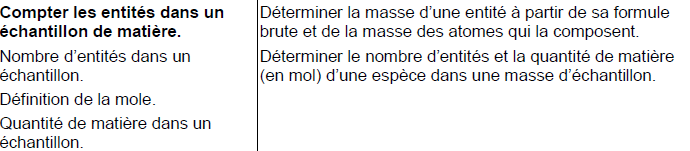
\includegraphics[width=1\textwidth]{BO.png}
\end{center}
}


\doc{2}{Exercices dans le livre scolaire}{
		\begin{enumerate}
			\item Compétence de base : exercice 5 page 65
			\item Pour confirmer : exercice 6, 16, 17 et 23 page 66-67
			\item Parcours expert : exercices 27, 29 et 30 page 69
		\end{enumerate}
}
	\noindent \textbf{Quiz sur la quantité de matière}
\begin{center}
	\begin{minipage}{.2\textwidth}
		\centering
		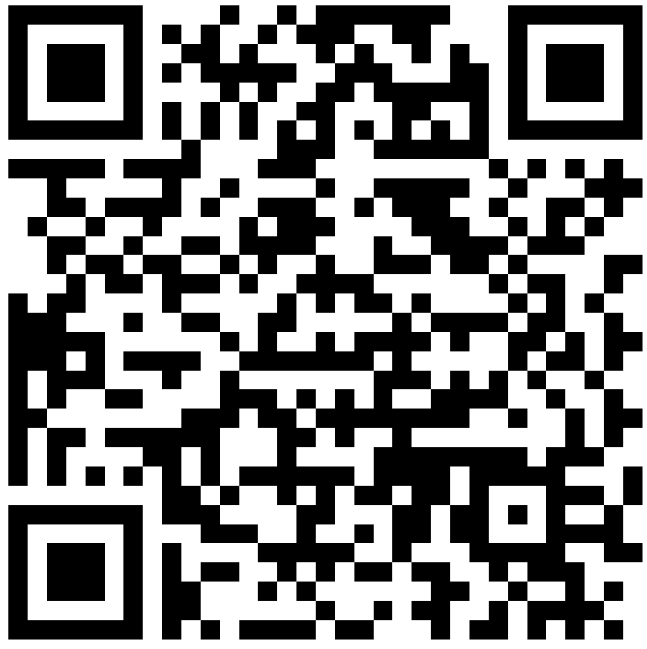
\includegraphics[width=.6\textwidth]{Quiz1.png}

		\protect Quiz 1 - La masse des entités : \url{https://forms.office.com/r/P15bbsP7b5}
	\end{minipage}
	\begin{minipage}{.2\textwidth}
		\centering
		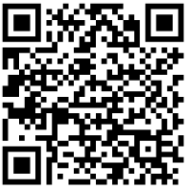
\includegraphics[width=.6\textwidth]{Quiz2.png}

		Quiz 2 - La quantité de matière : \url{https://forms.office.com/r/ByjFb92pwe?origin=lprLink}
	\end{minipage}
\end{center}
	% \begin{minipage}{.3\textwidth}
	% 	\centering
	% 	
\includegraphics[width=.7\textwidth]{Quiz3.png}

	% 	Quiz 3 : La caractéristique d'un dipôle : \hfill \url{https://forms.office.com/r/7vP0pmcU7Z}
	% \end{minipage}
% \begin{figure}[ht]
% 	% \centering
% 	\subfloat[Quiz 1 - Les circuits électriques : \hfill \url{https://forms.office.com/r/rLk3haXCTN}]{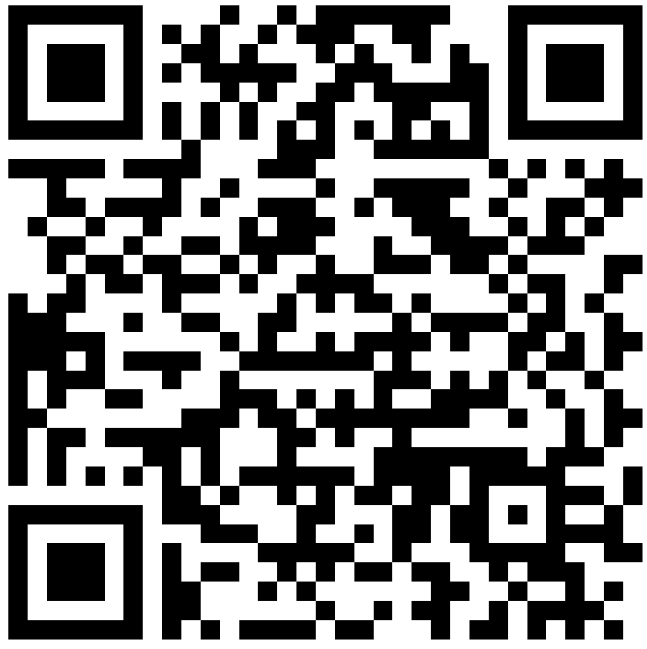
\includegraphics[width=.2\textwidth]{Quiz1.png}}\hfill
% 	\subfloat[Quiz 2 - Les lois de Kirchoff : \hfill \url{https://forms.office.com/r/JWeK6W4iiY?origin=lprLink}]{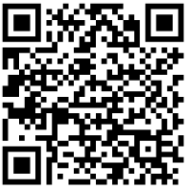
\includegraphics[width=.2\textwidth]{Quiz2.png}}\hfill
% 	\subfloat[Quiz 3 : La caractéristique d'un dipôle : \hfill \url{https://forms.office.com/r/7vP0pmcU7Z}]{
\includegraphics[width=.2\textwidth]{Quiz3.png}}\hfill
% 	% \subfloat[Pour aller plus loin : \hfill \url{https://learningapps.org/view23412425}]{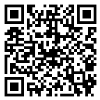
\includegraphics[width=.2\textwidth]{PourAllerPLusLoin.png}}\hfill

% % \end{figure}

% \clearpage
\section*{Introduction}

Nous avons étudié la matière à l’échelle macroscopique, puis à l’échelle microscopique.
Dans ce chapitre, nous créons un lien entre ces deux échelles, en comptant
les entités chimiques présentes dans un échantillon.

\section{Consitution de la matière}
\begin{center}
	\textit{ref : le livre scolaire page 61}
\end{center}

\subsection{À l'échelle microscopique}


\begin{definition}{Définition 1 - Trois majeures structures chimiques}

	À l'échelle microscopique, il faut considérer différents types de structures chimiques: 
	\begin{itemize}
		\item  La structure atomique (comme le fer);
		\item  La structure moléculaire (par exemple le sucre (saccharose $\rm C_{12}H_{22}O_{11}$));
		\item  La structure ionique avec des ions positifs appelés cations et des ions négatifs appelés anions ($Na^+$ et $Cl^-$ dans une eau salée).
	\end{itemize}	
\end{definition}

\subsection{À l'échelle macroscopique}

\begin{itemize}
	\item Quel est l'ordre de grandeur de la masse d'une entité chimique ? \medskip

		La masse d'une entité chimique est de l'ordre de $10^{-26}~\rm kg.$
\end{itemize}

\begin{definition}{Définition 2 - Espèce chimique à l'échelle macroscopique}

	Ce qui définit une espèce chimique au niveau macroscopique c'est à dire à notre échelle, dépend de l'entité microscopique qui la compose.
\end{definition}

\subsection{Le cas particulier des composés ioniques}

\begin{definition}{Définition 3 - Un composé ionique}
	\medskip

	On appelle composés ioniques des corps constitués d'ions liés entre eux par des interactions électrostatiques.\medskip

	Mis en solution dans l'eau, ces composés ioniques se dissocient en cations (ions chargés $+$) et en anions (ions chargés $-$).\medskip

	L'électronetralité est vérifiée en permanence.
\end{definition}

\noindent \textbf{Donner deux exemples de composés ioniques}\medskip

$\bullet$ le sel de table $(\rm Na^+, Cl^-)$.\medskip

$\bullet$ le sulfate d'aluminium $\rm Al_2(SO_4)_3$.


\section{Nombre d'entités dans un échantillon}

\subsection{Masse d'une entité chimique}

\begin{definition}{Définition 3  - Masse d'un atome (Rappel)}
	La masse d'un atome et l'ion monoatomique correspondant est pratiquement égale à celle de leur noyau. 

	\begin{equation}
		m_{\rm atome} = m_{\rm ion} = A\times m_{n}
	\end{equation}

	Où $A$ est le nombre de nucléons dans le noyau (nombre de masse) et $m_n$ la masse d'un seul nucléon.
\end{definition}

$\bullet$ \textbf{Comment calcule-t-on la masse d'une molécule ou d'un ion polyatomique (contenant plusieurs atomes) ?}\medskip

Il faut prendre en compte la masse de chaque entité chimique qui compose la molécule, ainsi que le nombre de ces entités chimiques. Par exemple pour la molécule de saccharose  $\rm C_{12}H_{22}O_{11}$ : 
$$m_{\rm totale} = 12\times m(C) + 22\times m(H) + 11\times m(O)$$

% \exo{2}{L'ammoniac $NH_3$ est une espèce chmique utilisée pour produire des engrais azotés.}{\noindent\textbf{Déterminer la masse d'une molécule d'ammoniac.} 

% \textit{Données : } $m_{\rm azote} = 2,33\times 10^{-26}~\rm kg$ et $m_{\rm hydrogène} = 1,67\times 10^{-27}~\rm kg$.

% \vspace{3cm}}

\exo{1}{Calcul de masses}{
	\begin{enumerate}
		\item Calculer la masse d'un atome d'hydrogène ($A=1$), puis celle d'un atome d'oxygène (A = 16). On rappelle que $m_{\rm nucléon} = 1,67\times 10^{-27}~\rm kg$
		\item Calculer, en kg, la masse d'une molécule d'eau $\rm H_2O$
		\item Calculer, en kg, la masse d'un ion hydroxyde $\rm HO^{-}$.
	\end{enumerate}

	\noindent \textbf{Solution:}

	\begin{enumerate}
		\item La masse d'un atome d'hydrogène $m_{H} = 1\times m_{\rm nucléon} = 1,67\times 10^{-27}~\rm kg$. la masse d'un atome d'oxygène $m_O=16\times 1,67\times 10^{-27} = 2.6\times 10^{-26}~\rm kg$.
		\item Masse d'une molécule d'eau $m_{\rm H_2O} = 2m_H + m_O = 3,00\times 10^{-26}~\rm kg$.
		\item Masse d'un ion hydroxyde $m_{\rm HO} = m_H+m_O = 2,84\times 10^{-26}~\rm kg$.
	\end{enumerate}
}

\subsection{Nombre d'entités chimiques}

Une espèce chimique est formée d'un nombre considérable d'entités chimiques identiques noté $N$.

\begin{definition}{Définition 4 - Nombre d'entités}
	Connaissant la masse $m$ d'un échantillon d'une espèce et celle de l'entité $m_{\rm entité}$, on détermine par proportionnalité, le nombre d'entité $N$:

	\begin{equation}
		N = \dfrac{m_{\rm échantillon}}{m}
	\end{equation}
\end{definition}
\clearpage
\exo{2}{Atomes de diamant}{Le diamant est un minéral entièrement constitué d'atomes de carbone \isotope{12}{6}{C} (la même matière qu'un morceau de charbon ou de mine de crayon gris 1 ).

\begin{center}
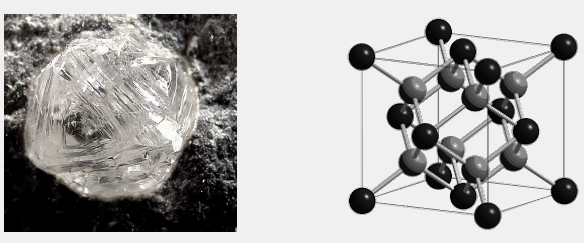
\includegraphics[width=.7\textwidth]{diamant.png}

\textit{À gauche un diamant brut, à droite l'arrangement microscopique des atomes de carbone dans un diamant.}
\end{center}
\begin{enumerate}
	\item Calculer la masse d'un atome de carbone \isotope{12}{6}{C}. On rappelle que $m_{\rm nucléon} = 1,67\times 10^{-27}~\rm kg$.
	\item Calculer le nombre d'atomes que comporte un diamant de $0,2~\rm g$. 
	\item Un tel diamant coûte environ 15000 \euro{}. Quel est le prix d'un atome de diamant ? Commenter. 
\end{enumerate}
	\noindent \textbf{Solution:}

\begin{enumerate}
	\item $m(\isotope{12}{6}{C}) = 12 \times m_{\rm nucléon} = 12 \times 1,67\times 10^{-27} = 2,00 \times 10^{-26}~\rm kg$.
	\item $N = \dfrac{m_{\rm totale}}{m_{\rm 1~atome}} = \dfrac{0,2\times 10^{-3} (\rm kg)}{2,00\times 10^{-26}(\rm kg)} = 1,0 \times 10^{22}~\rm atomes$ dans un diamant de 0,2 grammes.
	\item Un atome coûte $\dfrac{15000}{N} = \dfrac{15000}{1,0\times 10^{22}} = 1.5\times 10^{-18} $\euro{}.
\end{enumerate}
}

\vspace{.1cm}
\section{Quantité de matière}
\vspace{-.3cm}
Les échantillons de matière que l'on manipule au quotidien contiennent un
nombre d’entités chimiques colossal, comme l’a montré l'\bsc{exercice 2}. Afin de faciliter leur comptage, on regroupe ces entités par paquets.

\begin{figure}[ht]
	\centering
	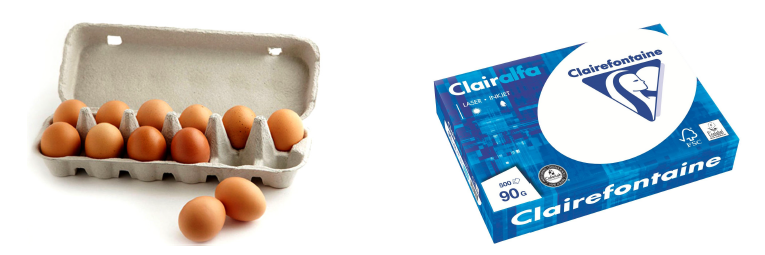
\includegraphics[width=.35\textwidth]{viecourante.png}	
	\caption{Boîte de 12 \oe ufs à gauche, ramette de feuilles de papier à droite.}
\end{figure}

On procède souvent de la même manière dans la vie courante, par exemple : 
\begin{itemize}
	\item On ne compte pas les \oe ufs un par un, mais par boîtes d'\oe ufs. 
	\item L'intendant du lycée n'achète pas les feuilles de papier une par une, mais par ramettes de 90 feuilles.
\end{itemize}

\subsection{La constante d'Avogadro}

\begin{minipage}{.3\textwidth}
	Afin de compter les entités, on les regroupera par
paquets de $\mathcal{N}_A$ , où $\mathcal{N}_A$ est un nombre appelé constante d'\bsc{Avogadro} ; en hommage au scientifique Italien Amedeo Avogadro (1776 - 1856) qui, le premier, distingua les atomes des molécules.\bigskip

On appelle la mole un paquet de $\mathcal{N}_A$ entités chimiques.
\end{minipage}\hspace{.5cm}
\begin{minipage}{.12\textwidth}
	\histo{Amedeo Avogadro}{
		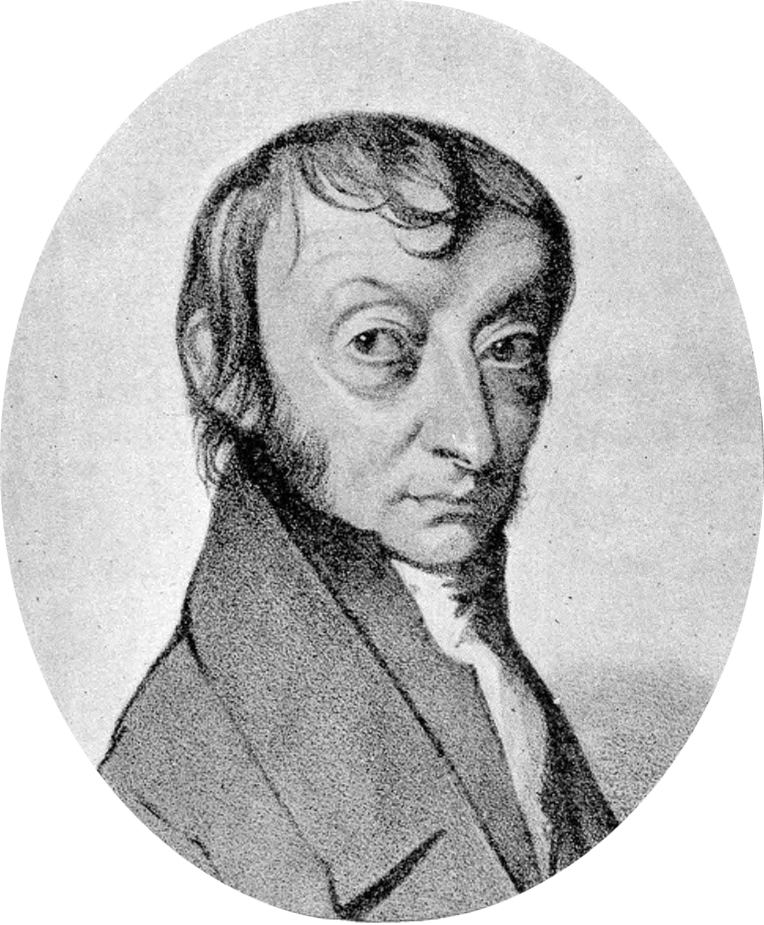
\includegraphics[width=1\textwidth]{Avogadro_Amedeo.jpg}
	}
\end{minipage}
% \medskip

\begin{definition}{Définition 5 - constante d'\bsc{Avogadro}}

Chaque mole contient un nombre définit d'entités chimiques : 

$$\mathcal{N}_A = 6,022\times 10^{23}~\rm mol^{-1}$$

Ce nombre s'appelle nombre d'Avogadro. 
\end{definition}


\subsection{L'unité de quantité de matière : la mole}

Le nombre d'entités $N$ est généralement très grand, pour compter le nombre d'entités il est plus aisé d'imaginer des boîtes de rangement dans lesquelles on range les entités chimiques.

\begin{definition}{Définition 6 - La quantité de matière}
	\medskip

	En chimie, ces boîtes s'appellent des moles.\medskip
	
	Son symbole est $n$. Elle s'exprime en mol. 
\end{definition}

\begin{Proposition}{Propriété 1 - Expression de la quantité de matière}
	Il y a proportionnalité entre $n$ et $N$, on a : 

	$$n=\dfrac{N}{\mathcal{N}_A}$$
\end{Proposition}

\exo{3}{Quantité de matière}{
	\begin{enumerate}
		\item Calculer la quantité de matière de carbone $n_c$ présente dans le diamant de l'exercice 2.
		\item Une bague de platine contient une quantité $n_{Pt} = 50\times 10^{-3}~\rm mol$ de platine. Quel nombre d'atomes de platine N cela représente-t-il ? 
	\end{enumerate}

	\noindent \textbf{Solution:}

	\begin{enumerate}
		\item $$n= \dfrac{N}{\mathcal{N}_A} = \dfrac{1,0\times 10^{22}}{6,022\times 10^{23}} = 1,7\times 10^{-2}~\rm mol$$
		\item $$N = n\times \mathcal{N}_A = 50\times 10^{-3}\times 6,022\times 10^{23} = 3,01\times 10^{22}$$ atomes de platine dans une bague.
	\end{enumerate}
	
}
\begin{center}
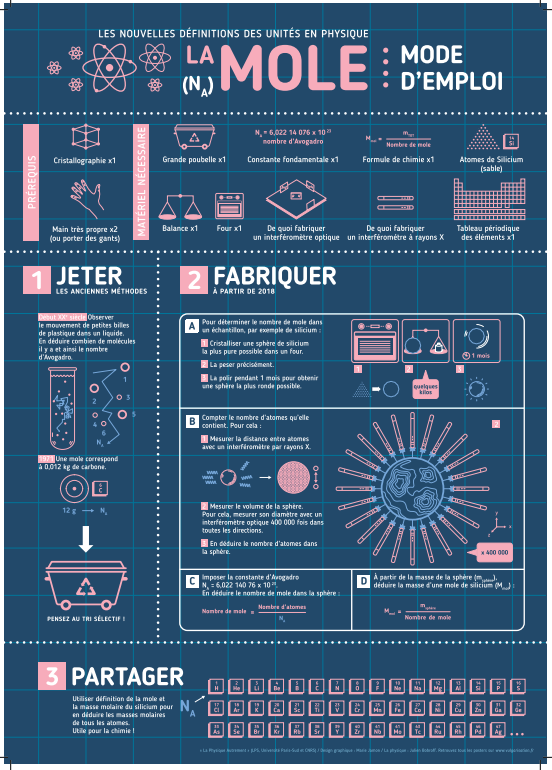
\includegraphics[width=.35\textwidth]{Lamole.png}
\end{center}
\end{document}

%%
%% FIN DU DOCUMENT
%%
